\documentclass[conference,letterpaper]{IEEEtran}
\IEEEoverridecommandlockouts
\usepackage[T1]{fontenc}
\usepackage[utf8]{inputenc}
\usepackage{newtxtext,newtxmath}
\usepackage{booktabs,tabularx,array,amsmath,multirow,float}
\usepackage{tikz}
\usetikzlibrary{positioning,arrows.meta}
\usepackage{url}
\usepackage[hidelinks]{hyperref}
\usepackage{microtype}
\usepackage{xcolor}
\setlength{\parskip}{1.4pt}
\linespread{1.045}
\renewcommand{\arraystretch}{1.16}
\newcommand{\stE}{\textsf{E}}
\newcommand{\stP}{\textsf{P}}
\newcommand{\stU}{\textsf{U}}
\newif\ifblind
\blindfalse
\begin{document}
\title{From AI Strategy to University Rules in the GCC}
\author{}
\maketitle
\begin{abstract}
How can readers tell which official AI-governance documents govern a university activity, rather than merely express national ambition? We present the Four-Layer Public-Evidence Audit (4L-PEA) for six Gulf Cooperation Council (GCC) jurisdictions: national direction (L1), cross-sector controls (L2), higher-education-applicable controls (L3), and institutional rules (L4). Dated official records are coded explicit (E), partial (P), or unlocated (U) under layer-specific gates. In a retrospectively recovered 36-record source register with a 23 July 2026 document-date cutoff, L3=E in one jurisdiction and L4=E in six; a selected 57-institution panel yields 20 E, 12 P and 25 U. The study makes the unequal L3/L4 thresholds explicit. A worked UAE example, linked official clauses, a four-step workflow and editable audit forms make the protocol reusable. Two independent Oman institutional sources show why deleting one anchor from the 36-record register is not equivalent to withdrawing all L4 evidence in a separate institution panel. The interval representation of P is descriptive, not a measure of undiscovered sources or coder accuracy. Exact historical website visibility, the complete original eligibility universe, and independent intercoder reliability are not established. The contribution is a transparent, bounded documentary audit, not a claim of policy transmission or implementation.
\end{abstract}
\begin{IEEEkeywords}
AI governance, GCC, higher education, bilingual document audit, public traceability, evidence admissibility, policy reuse.
\end{IEEEkeywords}

\section{Why This Audit Is Needed}
An instructor needs to know whether AI use is permitted in an assignment, what must be disclosed, and who verifies a student's work. A national strategy can express ambition without answering those questions. The practical research question is therefore narrower than ``Which country has the best AI governance?'': \emph{Which official documents can a reader actually locate and check at each governance level?}

Prior studies have compared GCC national strategies~\cite{albous} and university AI policies across 40 universities in six global regions~\cite{jin}, 116 US research institutions~\cite{mcdonald}, and 343 institutions in five countries~\cite{parker}. Work on assessment~\cite{moorhouse}, university policy development~\cite{li}, and systematic or institution-level governance~\cite{jiang,khoza,an,bacalso,qian} illustrates substantial policy variety. Multi-level governance and policy translation are distinct concepts~\cite{vukasovic,donina}. Our contribution is the Four-Layer Public-Evidence Audit (4L-PEA), a \emph{source-to-claim procedure}: it shows how to record the evidence for four levels without assuming that a policy at one level caused, authorized, or was implemented by another.

\textbf{A reader example.} Suppose a ministry advertises AI innovation, while a university publishes a formal rule specifying allowed assistance in assessments. The ministry announcement can document ambition but cannot tell the student what that university permits. Our audit asks two different questions: \emph{does an HE-specific, operative instrument exist at the sector level?} and \emph{does a university-issued rule exist at a named institution?} It records direct textual evidence for each answer. It never assumes that one document caused the other or that staff comply with the document simply because it is online.

The cutoff applies to the document corpus, not to the publication dates of the 2026 scholarship used for context. The paper answers three questions: (1) Which layers contain a qualifying public instrument? (2) Does the difference between sector-level HE evidence and institutional rules persist under stated evidence and sampling changes? (3) What minimum record would enable another researcher to check each classification? The accompanying material gives that reader a workflow, not a new country score.

\section{The Four-Layer Decision Rule}
\subsection{What E, P and U mean}
For each GCC jurisdiction $j$ and layer $\ell$, record one nominal state $L_{\ell j}\in\{\stE,\stP,\stU\}$. \textbf{E (explicit)} needs a dated, inspectable official instrument meeting the layer's authority, scope and content gate. \textbf{P (partial)} is relevant official evidence that fails at least one gate; record a reason code: \emph{A} (not adopted), \emph{S} (wrong/narrow scope), \emph{C} (insufficient AI-use controls), or \emph{V} (unresolved version/date). \textbf{U (unlocated)} means no qualifying document was found by the recorded search, \emph{not} that no internal rule exists. Reason codes organize uncertainty; they were not retrospectively recoded for all 57 cases.

\begin{table}[H]
\centering\caption{A short rulebook for deciding whether evidence is explicit}
\label{tab:gates}\small
\begin{tabularx}{\columnwidth}{@{}p{0.1\columnwidth}X@{}}
\toprule
Level & To record \stE, the official document must show:\tabularnewline\midrule
L1 & Adopted or authoritative \emph{national AI direction}.\tabularnewline
L2 & An inspectable \emph{cross-sector operational} AI control, standard, regulation or guideline.\tabularnewline
L3 & \emph{HE-applicable sector guidance} that actually specifies AI-use controls (not only readiness metrics).\tabularnewline
L4 & \emph{At least one university/college rule} with institutional authority and applicable AI-use provisions.\tabularnewline
\bottomrule
\end{tabularx}
\end{table}

\textbf{The L3/L4 thresholds answer different questions.} L3 concerns the existence of an HE-sector instrument; L4 asks only whether \emph{one institution} has an applicable rule. L4=E does not mean that most universities have a policy. Conversely, the absence of a qualifying public L3 document does not invalidate an L4 rule. The mismatch is a comparison of two different, explicitly stated \emph{document-availability propositions}, not an estimate of sector compliance.

\subsection{Availability, documentary links and real use are separate}
Do not conflate three propositions: \emph{document availability}, \emph{an explicit inter-instrument link} (named citation/delegation in a clause), and \emph{observed implementation}. \textbf{Only document-layer states were coded}; no edges or actual practice were measured. Thus E/E/E/E does not prove a transmitted policy chain.

\begin{figure*}[t]
\centering
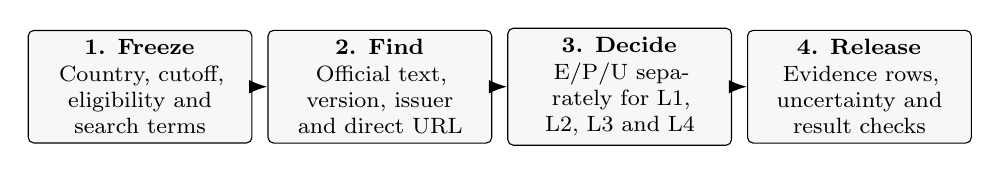
\begin{tikzpicture}[>=Latex, node distance=0.19cm, every node/.style={align=center}, box/.style={draw=black,rounded corners=2pt,minimum height=0.77cm,text width=0.215\textwidth,fill=black!3,font=\footnotesize}]
\node[box] (a) {\textbf{1. Freeze}\\ Country, cutoff, eligibility and search terms};
\node[box,right=of a] (b) {\textbf{2. Find}\\ Official text, version, issuer and direct URL};
\node[box,right=of b] (c) {\textbf{3. Decide}\\ E/P/U separately for L1, L2, L3 and L4};
\node[box,right=of c] (d) {\textbf{4. Release}\\ Evidence rows, uncertainty and result checks};
\draw[->,thick] (a)--(b);
\draw[->,thick] (b)--(c);
\draw[->,thick] (c)--(d);
\end{tikzpicture}
\caption{Four-step \emph{research workflow}. Arrows show audit steps, \textbf{not} causal transmission from national strategy to university policy. Black-and-white printing preserves all labels.}\label{fig:workflow}
\end{figure*}

\subsection{What the 23 July 2026 cutoff does and does not prove}
The primary frame uses instruments \emph{dated or operative no later than} 23 July 2026, including some located retrospectively. For each record, keep three distinct dates: \emph{issue/effective date}, \emph{first verifiable public-posting date}, and \emph{research retrieval date}. A pre-cutoff issue date alone does not prove public web availability at the cutoff. Unless a contemporaneous posting or archived capture verifies that fact, label it \emph{historical-public-availability unverified}. The published counts are conditional on the retained document and coder states, \emph{not} an independent snapshot of the web on 23 July.

\section{How to Apply the Method}
Figure~\ref{fig:workflow} is a reusable procedure for a country, education system or group of institutions. \textbf{Step 1: freeze} the decision question, document cutoff, official institutional frame, language scope and exact search terms \emph{before} seeing the outcome. \textbf{Step 2: locate} government, regulator, ministry and university texts, using the original document rather than a search snippet; record issuer, title, version, date, language, URL and pinpoint clause. \textbf{Step 3: code} each layer using Table~\ref{tab:gates}; keep any explicit cross-document citation in another field and never fill gaps by inference. \textbf{Step 4: report} all E/P/U states, missing evidence, sensitivity to disputed boundaries and raw source records. The reusable blank log and bilingual query templates accompany the PDF; they are \emph{prospective templates}, not a claim that every original search string was historically retained.

For a U closure, search Arabic and English on the institution's domain, policy library, assessment pages, handbook and integrity rules, recording every completed surface, query and date; a later discovery is logged separately. A ministry announcement that guidance is under development can be P; it is not automatically an enacted HE control. If Arabic and English editions disagree, record the scope, controlling-language clause and version authority and flag the classification for adjudication, rather than silently choosing a convenient translation. This is especially relevant where an English text is identified as a translation of an Arabic original~\cite{qataru}.

\subsection{Worked example: how the same country can have E, E, P, E}
The UAE provides a concise worked classification under the fixed cutoff:
\begin{center}
\small\setlength{\tabcolsep}{4pt}
\begin{tabularx}{\columnwidth}{@{}p{0.08\columnwidth}Xc@{}}
\toprule
Layer & Located official instrument / decision reason & State\\\midrule
L1 & UAE AI Strategy 2031: national direction~\cite{uaestrategy} & E\\
L2 & UAE AI Charter: cross-sector principles~\cite{uaecharter} & E\\
L3 & OBEF v11.5: AI-readiness metrics, not operative use controls~\cite{obef} & P\\
L4 & UAEU student GenAI use policy: a university rule~\cite{uaeupolicy} & E\\\bottomrule
\end{tabularx}
\end{center}
The profile is \textbf{E/E/P/E}. It says what is publicly \emph{documentable}, not that the university policy was caused by the evaluation framework. Under an explicitly broader \emph{evaluation-framework} threshold, UAE L3 changes to E; this decision is reported separately as sensitivity, never as a silent recode. The classification was not independently adjudicated by two coders.

\section{The GCC Evidence Frame}
The fixed source date is \textbf{23 July 2026}. The original 36-record register comprises seven L1, eight L2, five L3, eleven L4, and five GCC-regional records. Nineteen records have an Arabic and English location, fifteen an English location only, and two an Arabic location only. The register's document titles, issuer, date, locator and classification rationale are available online, but the full set of verbatim excerpts and independent archival hashes has \emph{not} been reverified for this revision. Source recovery is not retrospectively presented as a fresh complete search.

The jurisdictional L4 finding requires only one qualifying university. We added a \emph{separate, nonrandom corroboration panel}: officially recognized or licensed civilian HEIs, grouped by G1 public/general, G2 private/non-government and G3 public applied/specialized. The declared oldest-four-with-ties rule was applied inside each country--stratum cell, retaining smaller cells and excluding author-affiliated institutions before AI-policy search. The founding year is a selection variable, not a maturity score; selecting older institutions can favor better preserved web archives and limits generalizability.

Two eligibility corrections changed the selected members without changing that rule: a historical Bahrain regulator source placed Kingdom University in its eligible cell~\cite{bqa1,bqa2}; UAE accreditation evidence established Emirates Institute for Banking and Financial Studies (EIBFS) as an eligible older private institution, displacing two later cases~\cite{caa1,caa2}. The corrected panel is \textbf{57 institutions}. Importantly, the complete original pre-outcome eligible universe was not retained. The 57 are a \emph{retrospectively corrected selected panel}, not a reconstructed fully frozen sampling frame. The companion workbook distinguishes known selection evidence from blank prospective full-frame forms; it is not a reconstructed original frame.

\section{Results: What the Documents Show}
\begin{table*}[t]
\centering\caption{GCC results at the fixed cutoff: four documentary states and the independent 57-institution corroboration counts. The last three columns are \emph{selected-case counts}, not national prevalence rates.}
\label{tab:core}\small
\setlength{\tabcolsep}{6pt}
\begin{tabularx}{\textwidth}{@{}p{0.185\textwidth}ccccrrrX@{}}
\toprule
Jurisdiction & L1 & L2 & L3 & L4 & E & P & U & How to interpret\tabularnewline\midrule
United Arab Emirates & E & E & P & E & 5 & 3 & 5 & HE OBEF is a sector evaluation framework, not an L3 control under primary gate.\tabularnewline
Saudi Arabia & E & E & E & E & 3 & 4 & 4 & Four gates have visible instruments; no transfer claim is made.\tabularnewline
Qatar & E & E & P & E & 2 & 2 & 6 & University rules visible despite partial L3 evidence.\tabularnewline
Oman & E & E & U & E & 2 & 1 & 5 & SQU source has version HOLD; Majan handbook corroborates L4~\cite{squ,majanhb}.\tabularnewline
Bahrain & P & E & U & E & 6 & 0 & 1 & School-oriented initiative does not qualify as HE-specific L3~\cite{bahrain}.\tabularnewline
Kuwait & P & P & U & E & 2 & 2 & 4 & Kuwait University rule provides an L4 example.\tabularnewline\midrule
\textbf{Total (selected HEIs)} & & & & & \textbf{20} & \textbf{12} & \textbf{25} & \textbf{57 cases across six states}.\tabularnewline\bottomrule
\end{tabularx}
\end{table*}

Table~\ref{tab:core} makes the main result visible without a color-coded country score. National AI direction is E in four states, operational governance in five, HE-sector controls in one and an institution-level rule in all six. In \emph{five of six states}, a visible L4 rule coexists with an L3 state other than E. Define the descriptive count
\begin{equation}\label{eq:d}
D=\#\{j:L_{4j}=\stE\ \text{and}\ L_{3j}\neq\stE\}=5.
\end{equation}
A higher level's partial or unlocated public documentation cannot be interpreted as proof of a broken regulation or of institutional non-compliance. The 57-case panel contains \textbf{20 E, 12 P and 25 U}; each country has at least two E and at least one non-E case. They show observable diversity within a \emph{purposefully selected panel}; the fractions 20/57, 12/57 and 25/57 are \emph{not representative population estimates}. The full 57-row links remain in the supplement instead of a micro-font table.

\subsection{What changes when a source or rule changes?}
\begin{table}[H]
\centering\caption{Explicitly scoped sensitivities; $D$ is a count, displayed as $D/N$}
\label{tab:sensitivity}\small
\setlength{\tabcolsep}{3pt}
\begin{tabularx}{\columnwidth}{@{}Xccc@{}}
\toprule
Scope / scenario & L3 E & L4 E & $D/N$\tabularnewline\midrule
Primary 36-record chain & $1/6$ & $6/6$ & $5/6$\tabularnewline
Remove SQU \emph{only from 36-record chain} & $1/6$ & $5/6$ & $4/6$\tabularnewline
Include Majan L4 in Oman fallback\footnotemark & $1/6$ & $6/6$ & $5/6$\tabularnewline
Broader UAE OBEF scope & $2/6$ & $6/6$ & $4/6$\tabularnewline
Leave out Saudi Arabia & $0/5$ & $5/5$ & $5/5$\tabularnewline
Leave out any other state & $1/5$ & $5/5$ & $4/5$\tabularnewline\bottomrule
\end{tabularx}
\footnotetext{Cross-panel evidence union, \emph{not} the original 36-record-only leave-one-source calculation. The 57-HEI panel codes Majan as E from its 2025--26 handbook, \S5.7.7~\cite{majanhb,majannews}.}
\end{table}

\textbf{The Oman diagnostic needs two scopes.} Removing Sultan Qaboos University (SQU) from the \emph{36-record register only} makes that register's Oman L4 unlocated; it does \emph{not} eliminate a second qualifying Oman L4 source in the \emph{separate 57-institution panel}. Majan University College's 2025--26 official handbook \S5.7.7 gives institution-wide student assessment rules, including permitted study support, restrictions on submitted work and disclosure, and the college announced the handbook publicly on 20 October 2025~\cite{majanhb,majannews}. Retaining Majan as an L4 fallback keeps Oman E. These calculations test different source universes; neither estimates implementation. Broadening the UAE OBEF gate reduces $D$ to four by changing a \emph{sector} judgment~\cite{obef}.

A brief P-only interval representation is reported in the companion guide~\cite{petry,pekala}: $F_3=[1/6,3/6]$, $F_4=[1,1]$, minimum difference $1/2$. This is algebra from the categorical states, not measured coder uncertainty, missing-source coverage, or confidence intervals.

\subsection{Pinpoint checks on decisive public texts}
The frozen Saudi L3=E record SAU03 labels SDAIA's \emph{Generative AI in Education} as 2024, while SDAIA's public catalog dates a similarly titled entry 19 Nov. 2023~\cite{sdaiacat}. Edition identity and the exact decisive passage remain unverified. A second official instrument, the National eLearning Center's \emph{Regulations and Guidelines for the Use of GenAI Tools and Applications in Digital Learning} (v1.0), defines educational institutions to include universities/colleges (p. 3) and gives explicit institutional, assessment and disclosure controls (pp. 4--7)~\cite{nelcguide}. Its release is reported in the center's 2024 annual report~\cite{nelcreport}. This is \emph{additional source corroboration}, not a retroactively inserted 37th record; the SAU03 year/edition and passage gate remains open to independent adjudication.

For a second bilingual authority example, Qatar University's presidential instructions were approved and effective 25 Dec. 2025. Article 3 specifies disclosure and related controls (pp. 3--4); the official English edition expressly gives precedence to Arabic if text differs~\cite{qataru}. These pinpoint citations illustrate an E decision; they do not establish independent double coding. SQU's official policy index lists a GenAI teaching and assessment guide, but its precise authoritative version/effective date still needs separate source closure~\cite{squ}.

\section{What Another Researcher Can Reuse}
For a fully replayable audit, a reader must move from each claim back to its governing clause, not just its homepage. Every new audit should release: \textbf{(i)} a source register with issuer, edition, issue/effective date, language, document URL, exact clause and layer-specific decision; \textbf{(ii)} an eligibility list showing institutions included, excluded and tied at the boundary; and \textbf{(iii)} an E/P/U decision sheet with search/closure dates, explicit uncertainty flags and code that recalculates tables. An open hyperlink alone cannot substitute for the controlling provision or its date. A source URL that merely records an unsuccessful U search must be labelled as a \emph{search locator}, not cited as a positive policy.

For university staff, we propose \emph{eight public-rule questions}: who approved the operative version; whom it covers; what AI use is allowed in assessments; when disclosure is required; which tools or data are restricted; who verifies outputs; how fairness and appeals work; and who maintains future revisions. These fields address recurring traceability questions and align with general UNESCO/OECD governance concerns~\cite{unesco,oecd}. They are a \emph{documentation proposal}, not a validated policy-quality score. The companion field guide and editable worksheet turn each question into a source-linked check with blank evidence cells.

\ifblind
\noindent\textbf{Supplementary materials.} An anonymous companion PDF presents the 57-institution evidence/search key, plus a practical source-coding and bilingual search template. For review-stage anonymity, repository ownership information is omitted here; author-identifying archival links will be added only if permitted by the venue.
\else
\noindent\textbf{Supplementary materials and code.} The \href{https://github.com/shaikhamalkawi-ux/From-AI-Strategy-to-University-Rules-in-the-GCC/blob/main/ICAMAC2026_Paper90_R5_57/supplement/ICAMAC_Paper90_R5_Evidence_Addendum_FieldGuide_and_57.pdf}{\textbf{field guide and 57-institution linked appendix (PDF)}} is available with the \href{https://github.com/shaikhamalkawi-ux/From-AI-Strategy-to-University-Rules-in-the-GCC/tree/main/ICAMAC2026_Paper90_R5_57}{\textbf{version-matched research archive}} (57-case CSV, six-state matrix, provisional 36-source register, blank audit template and result checks). This is an author-linked archive; the supplement includes prospective templates and selected records, but not a completed independent replay.
\fi

\section{Limits and Conclusion}
The results concern \emph{public document availability at a declared cutoff}. They do not measure instrument-to-instrument transmission, implementation effectiveness, policy quality, causation, regional prevalence or missing-source rates. The historical search log is incomplete for exact independent replay; the 36-source register is provisional and only selected decisive-source checks have been freshly corroborated. The 57-case membership remains subject to a full original-frame completeness check. The E/P/U states were not independently double-coded, so no inter-rater agreement or Arabic--English adjudication rate is claimed. A future verification round should freeze source copies, use two independent coders, report a confusion matrix and agreement, adjudicate conflicts with controlling passages and record any revised outcomes before publication. These are \emph{outstanding validations}, not completed experiments.

The result conditional on the frozen coding is simple: at least one documented university-level rule is identified in each GCC jurisdiction, while the distinct HE-applicable sector control gate is E in one (two under a broader UAE scope). The portable finding is the \emph{difference between visible evidence, explicit linkage and actual practice}, together with a reusable source-to-claim workflow. The accessible ledger and \href{https://github.com/shaikhamalkawi-ux/From-AI-Strategy-to-University-Rules-in-the-GCC/blob/main/ICAMAC2026_Paper90_R5_57/resources/ICAMAC_Paper90_R5_Reusable_Audit_Workbook.xlsx}{companion workbook} make the \emph{arithmetic and future audit procedure} reusable; full historical source recovery and independent coding remain outstanding.

\begin{thebibliography}{33}\footnotesize
\bibitem{albous} M. R. Albous, O. R. Al-Jayyousi, and M. Stephens, ``AI governance in the GCC states: A comparative analysis of national AI strategies,'' \emph{Journal of Artificial Intelligence Research}, vol. 82, pp. 2389--2422, 2025, doi: 10.1613/JAIR.1.17619.
\bibitem{jin} Y. Jin, L. Yan, V. Echeverria, D. Gasevic, and R. Martinez-Maldonado, ``Generative AI in higher education: A global perspective of institutional adoption policies and guidelines,'' \emph{Computers and Education: Artificial Intelligence}, vol. 8, p. 100348, 2025, doi: 10.1016/j.caeai.2024.100348.
\bibitem{mcdonald} N. McDonald \emph{et al.}, ``Generative artificial intelligence in higher education: Evidence from an analysis of institutional policies and guidelines,'' \emph{Computers in Human Behavior: Artificial Humans}, vol. 3, p. 100121, 2025, doi: 10.1016/j.chbah.2025.100121.
\bibitem{parker} L. Parker \emph{et al.}, ``Comparative analysis of artificial intelligence policies in universities across five countries,'' \emph{Discover Computing}, vol. 28, p. 267, 2025, doi: 10.1007/s10791-025-09745-5.
\bibitem{moorhouse} B. L. Moorhouse, M. A. Yeo, and Y. Wan, ``Generative AI tools and assessment: Guidelines of the world's top-ranking universities,'' \emph{Computers and Education Open}, vol. 5, p. 100151, 2023.
\bibitem{li} M. Li \emph{et al.}, ``A framework for developing university policies on generative AI governance: A cross-national comparative study,'' \emph{Studies in Higher Education}, 2026, doi: 10.1080/03075079.2026.2696496.
\bibitem{jiang} X. Jiang and Z. Abdullah, ``AI-enabled governance in higher education: A systematic review of applications, outcomes, and emerging implications,'' \emph{Frontiers in Education}, vol. 11, p. 1856440, 2026, doi: 10.3389/feduc.2026.1856440.
\bibitem{khoza} M. S. Khoza, S. F. Wamba, and S. Nyawa, ``Mapping the landscape of AI governance in higher education,'' \emph{Assessment \& Evaluation in Higher Education}, 2026, doi: 10.1080/02602938.2026.2712521.
\bibitem{an} Y. An, J. H. Yu, and S. James, ``Investigating higher education institutions' guidelines and policies regarding the use of generative AI in teaching, learning, research, and administration,'' \emph{International Journal of Educational Technology in Higher Education}, vol. 22, p. 10, 2025.
\bibitem{bacalso} F. D. Bacalso \emph{et al.}, ``Institutional approaches to generative AI management in higher education: A systematic review,'' \emph{Frontiers in Education}, vol. 11, p. 1814426, 2026, doi: 10.3389/feduc.2026.1814426.
\bibitem{qian} Y. Qian, ``Governing generative AI in higher education: Emerging policy approaches and support ecosystems at innovative U.S. universities,'' \emph{International Journal for Educational Integrity}, vol. 22, p. 25, 2026, doi: 10.1007/s40979-026-00233-x.
\bibitem{vukasovic} M.-H. Chou, J. Jungblut, P. Ravinet, and M. Vukasovic, ``Higher education governance and policy: An introduction to multi-issue, multi-level and multi-actor dynamics,'' \emph{Policy and Society}, vol. 36, no. 1, pp. 1--15, 2017, doi: 10.1080/14494035.2017.1287999.
\bibitem{donina} D. Donina and S. Hasanefendic, ``Higher education institutional governance reforms in the Netherlands, Portugal, and Italy: A policy translation perspective addressing the homogeneous/heterogeneous dilemma,'' \emph{Higher Education Quarterly}, vol. 73, no. 1, pp. 29--44, 2019.
\bibitem{squ} Sultan Qaboos University, Quality Assurance Office, ``Guidelines for using GenAI tools in teaching, learning and assessment,'' listed in institutional teaching and learning guides; precise version date not independently established. [Online]. Available: \url{https://www.squ.edu.om/qao/Policies-and-Procedures}.
\bibitem{obef} UAE Ministry of Higher Education and Scientific Research, ``University guidebook for outcome-based evaluation framework (OBEF), version 11.5,'' 23 Mar. 2026. [Online]. Available: \url{https://www.mohesr.gov.ae/Documents/OBF%20University%20Guide%20-%20EN.pdf}.
\bibitem{bqa1} Education and Training Quality Authority (BQA), Bahrain, ``Institutional review report: Kingdom University,'' 2019. [Online]. Available: \url{https://www.bqa.gov.bh/En/Reports/UniReports/HigherEducationReport/KU%20Inst%20en%20C2.pdf}.
\bibitem{bqa2} Education and Training Quality Authority (BQA), Bahrain, ``Higher education reports,'' 2026; index modified 7 July 2026. [Online]. Available: \url{https://www.bqa.gov.bh/institutions-performance/higher-education-reports/}.
\bibitem{caa1} Commission for Academic Accreditation, UAE, ``Renewal of licensure: Emirates Institute for Banking and Financial Studies---executive summary,'' 2019. [Online]. Available: \url{https://caa.ae/PORTALSUMMARYREPORTS/16/EIBFS%20Executive%20Summary.pdf}.
\bibitem{caa2} Commission for Academic Accreditation, UAE, ``Higher education institution: Emirates Institute for Banking and Financial Studies,'' 2026. [Online]. Available: \url{https://www.caa.ae/Pages/Institutes/Details.aspx?GUID=16}.
\bibitem{petry} F. E. Petry and R. R. Yager, ``Interval-valued fuzzy sets aggregation and evaluation approaches,'' \emph{Applied Soft Computing}, vol. 124, p. 108887, 2022.
\bibitem{pekala} B. P\k{e}kala, K. Dyczkowski, P. Grzegorzewski, and U. Bentkowska, ``Inclusion and similarity measures for interval-valued fuzzy sets based on aggregation and uncertainty assessment,'' \emph{Information Sciences}, vol. 547, pp. 1182--1200, 2021.
\bibitem{bahrain} Ministry of Education, Kingdom of Bahrain, ``Digital empowerment in education program,'' updated 30 Dec. 2025; school-sector target groups. [Online]. Available: \url{https://moe.gov.bh/en/digital-empowerment-in-education-program}.
\bibitem{unesco} UNESCO, \emph{Guidance for Generative AI in Education and Research}. Paris: UNESCO, 2023.
\bibitem{oecd} OECD, ``Policies supporting responsible and systematic GenAI adoption in higher education,'' \emph{OECD Education Spotlights}, no. 23, 2026, doi: 10.1787/c4e5621f-en.
\bibitem{qataru} Qatar University, ``Instructions on the use of generative artificial intelligence tools at Qatar University,'' approved/effective 25 Dec. 2025; English translation of Arabic original. [Online]. Available: \url{https://www.qu.edu.qa/en-us/about/policy/Documents/Instructions%20onThe%20Use%20of%20Generative%20Artificial%20Intelligence%20Tools%20at%20Qatar%20University-Approved.pdf}.

\bibitem{uaestrategy} UAE Government, ``UAE Strategy for Artificial Intelligence 2031,'' national AI policies and strategy portal. [Online]. Available: \url{https://u.ae/en/about-the-uae/digital-uae/digital-technology/artificial-intelligence/artificial-intelligence-in-government-policies}.
\bibitem{uaecharter} UAE Government, ``The UAE Charter for the Development and Use of Artificial Intelligence,'' 2024. [Online]. Available: \url{https://u.ae/en/about-the-uae/strategies-initiatives-and-awards/policies/Ai/The-UAE-Charter-for-the-Development-and-Use-of-Artificial-Intelligence}.
\bibitem{uaeupolicy} United Arab Emirates University, ``Generative AI Usage by the Students Policy,'' 2025. [Online]. Available: \url{https://www.uaeu.ac.ae/en/about/pdfs/policies-2025/generative-ai-policy.pdf}.
\bibitem{majanhb} Majan University College, \emph{Undergraduate Student Handbook 2025--2026}, \S5.7.7, p. 46. [Online]. Available: \url{https://move.majancollege.edu.om/mod/resource/view.php?id=90589}.
\bibitem{majannews} Majan University College, ``UG Handbook 2025--2026,'' official MOVE campus announcement, 20 Oct. 2025. [Online]. Available: \url{https://move.majancollege.edu.om/mod/forum/discuss.php?d=103095}.
\bibitem{sdaiacat} Saudi Data and Artificial Intelligence Authority (SDAIA), ``Generative AI in Education,'' official publications catalog, entry dated 19 Nov. 2023. [Online]. Available: \url{https://sdaia.gov.sa/en/MediaCenter/KnowledgeCenter/Pages/SDAIAPublications.aspx}.
\bibitem{nelcguide} Saudi National eLearning Center, \emph{Regulations and Guidelines for the Use of GenAI Tools and Applications in Digital Learning}, v1.0, pp. 3--7. [Online]. Available: \url{https://storage.googleapis.com/futurexcms/wthyqt_dwabt_En_0a523e42f5/wthyqt_dwabt_En_0a523e42f5.pdf}.
\bibitem{nelcreport} Saudi National eLearning Center, \emph{Annual Report 2024}, p. 64, reporting the launch of the GenAI digital-learning guide. [Online]. Available: \url{https://storage.googleapis.com/futurexcms/altqryr_alsnwy_alnskht_alielamyt_V4_hjm_aql_2024_d86ff6c8af/altqryr_alsnwy_alnskht_alielamyt_V4_hjm_aql_2024_d86ff6c8af.pdf}.
\end{thebibliography}
\end{document}
